\documentclass[english,notitlepage,letterpaper, 10pt]{article} % para articulo en castellano
\usepackage{cite}
\usepackage[utf8]{inputenc} % Acepta caracteres en castellano
\usepackage[spanish]{babel} % silabea palabras castellanas
\usepackage{amsmath}
\decimalpoint

\makeatletter
\renewcommand*\env@matrix[1][*\c@MaxMatrixCols c]{%
  \hskip -\arraycolsep
  \let\@ifnextchar\new@ifnextchar
  \array{#1}}
\makeatother

\usepackage{here}

\usepackage{amsfonts}
\usepackage{amssymb}
\usepackage{hyperref} % navega por el doc
\usepackage{graphicx}
\usepackage{geometry}      % See geometry.pdf to learn the layout options.
\geometry{letterpaper}                   % ... or a4paper or a5paper or ... 
%\geometry{landscape}                % Activate for for rotated page geometry
%\usepackage[parfill]{parskip}    % Activate to begin paragraphs with an empty line rather than an indent
\usepackage{epstopdf}
\usepackage{fancyhdr} % encabezados y pies de pg
\usepackage{mathtools}

\usepackage{listings}
\usepackage{color}

\definecolor{dkgreen}{rgb}{0,0.6,0}
\definecolor{gray}{rgb}{0.5,0.5,0.5}
\definecolor{mauve}{rgb}{0.58,0,0.82}

\lstset{frame=shadowbox,
  language=Matlab,
  aboveskip=3mm,
  belowskip=3mm,
  showstringspaces=false,
  columns=flexible,
  basicstyle={\small\ttfamily},
  numbers=left,
  numberstyle=\tiny\color{gray},
  keywordstyle=\color{blue},
  commentstyle=\color{dkgreen},
  stringstyle=\color{mauve},
  breaklines=true,
  breakatwhitespace=true
  tabsize=3
  rulesepcolor=\color{blue}
}

\newcommand{\university}{\normalsize Universidad Industrial de Santander}
\newcommand{\faculty}{\normalsize  Escuela de Ingenier\'ia de Sistemas e Inform\'atica}
\newcommand{\codigo}{\normalsize  2182066}
\newcommand{\grupo}{\normalsize  B2}
\pagestyle{fancy} 
\chead{\bfseries Lab. } 
\lhead{} % si se omite coloca el nombre de la seccion
\rhead{\today} 
\lfoot{\it  An\'alisis N\'umerico } 
\cfoot{\university} 
\rfoot{\thepage} 

\voffset = -0.25in 
\textwidth = 7.5in
\textheight = 9in
\oddsidemargin = -0.5in
\headheight = 20pt 
\headwidth = 7.5in
\renewcommand{\headrulewidth}{0.5pt}
\renewcommand{\footrulewidth}{0,5pt}
\DeclareGraphicsRule{.tif}{png}{.png}{`convert #1 `dirname #1`/`basename #1 .tif`.png}


\begin{document}

\title{	\vspace{-12mm}
\includegraphics[width=0.2\linewidth]{Logos/UIS.pdf}\\Informe Laboratorio: An\'alisis Num\'erico\\  \centering Pr\'actica No. 6}
\author{
  \textbf{Daniel Delgado} \\ \textbf{C\'odigo:} \codigo\\
  \textbf{Grupo:} \grupo\\
  \textit{\faculty}\\
  \textit{\university}}
\date{\today}
\maketitle

\section{Introducci\'on}

La interpolación, específicamente la interpolación polinómica, es una práctica la cual permite el encontrar más una función a partir de un conjunto de puntos dados. Esto puede ser por seguimiento de la tendencia de una función o la generación de un polinómio que se ajuste a un set de puntos dados.

En el presente informe, tratará las interpolaciones polinómicas de Newton y LaGrange además el como estas operan y se diferencian entre ellas. De la misma manera, se buscará entender el como cada una de estas se comporta en un contexto computacional y las ventajas respectivas.

La compresión de las diferentes maneras de realizar interpolaciones, al igual que el desarrollo de la algoritmia relacionada, son los principales temas a a tratar durante el desarrollo del presente informe, así como la resolución de los problemas propuestos a manera de pregunta orientadora del componente práctico del mismo.

\section{Desarrollo}

\begin{enumerate}
  
  \item Preguntas propuestas
  
    De manera inicial, la guía de trabajo plantea algunas preguntas base con el fin de establecer los conceptos básicos que serán trabajados a lo largo del desarrollo del presente informe.

    \begin{enumerate}
      \item ¿Qué es la interpolación?
      
      En términos simples, la interpolación se define como la obtención de puntos de una función indeterminada a partir de algunos puntos conocidos. Esto se hace comúnmente para la búsqueda de tendencias dadas por algunos datos o con el fin de realizar una aproximación de alguna función hacia algo más simple.

      \item ¿Cómo se calcula un polinomio del Taylor de grado N?
      
      Los polinomios de Taylor de grado N, aunque existen varias maneras de calcularlos, dentro de un dominio determinado $[a,b]$, es posible calcularlos a partir de la siguiente sumatoria la cual es usada para aproximar una función:

      \begin{center}
        \begin{math}
          f (x) \approx P (x) = \displaystyle\sum_{k=0}^{N} \frac{f^{(k)}(x)}{k!}(x-x_0)^k
        \end{math}
      \end{center}

      Es gracias a esto que podemos realizar aproximaciones polinómicas de algunas funciones más complejas como lo vienen siendo las funciones sinusoidales o exponenciales.

      \item ¿Cómo se calculan las interpolaciones de Newton y LaGrange?

      Estas interpolaciones son calculadas de dos maneras bastante diferentes diferentes pero toma datos similares para realizar este proceso.
      
      La interpolación de LaGrange se realiza en dos partes, la primera, es el cálculo de los productos de los puntos que serán usados para realizar la generación del polinómio:

      \begin{center}
        \begin{math}
          L_i(x) = \displaystyle\prod_{j=0, j \not= i}^{n} \frac{x-x_j}{x_i - x_j}
        \end{math}
      \end{center}

      Seguidamente, empleando los valores obtenidos para $L_i$, se calculará el polinómio resultante de la interpolación a partir de la siguiente sumatoria:

      \begin{center}
        \begin{math}
          f_n(x)  = \displaystyle\sum_{i=0}^n L_i(x)f(x_i)
        \end{math}
      \end{center}
      
      En cuanto a la interpolación de Newton, también conocida como diferencias divididas, es calculada a partir del siguiente proceso recursivo:

      \begin{center}
        \begin{math}
          \displaystyle f_i(x_0,x_1,x_2,...,x_{i-1},x_i) = \frac{ f_{i-1}(x_0,x_1,...,x_{i-1},x_i)-f_i(x_0,x_1,x_2,...,x_{i-1})}{x_i - x_0}
        \end{math}
      \end{center}

      \item ¿Qué aplicaciones tiene la interpolación?

      La interpolación tiene múltiples aplicaciones. Estas aplicaciones están principalmente relacionadas con la búsqueda de una función aproximada a partir de un polinómio de grado n. Estas aproximaciones pueden ser usadas principalmente para la simplificación de cálculos y la reducción de tiempos de computación para funciones donde la precisión no debe ser extremadamente alta.

    \end{enumerate}

    \item Aplicando
    
    \begin{enumerate}

      \item Para encontrar el polinomio cuadrático de LaGrange $P_2(x)$ para la función $y=f(x)=\sqrt{x}$, debemos  realizar siguiente sumatoria:

      \begin{center}
        \begin{math}
          P_n(x)  = \displaystyle\sum_{i=0}^n L_i(x)f(x_i)
        \end{math}
      \end{center}

      Con el fin de realizar esto, tenemos que encontrar los valores para $L_i(x)$ los cuales son obtenidos a partir del siguiente producto:

      \begin{center}
        \begin{math}
          L_i(x) = \displaystyle\prod_{j=0, j \not= i}^{n} \frac{x-x_j}{x_i - x_j}
        \end{math}
      \end{center}

      Partiendo de los valores para $x_i$ dados en el enunciado, podemos realizar el cálculo de $L_0(x)$, $L_1(x)$, $L_2(x)$:

      \begin{center}
        \begin{math}
          \displaystyle L_0(x) = \frac{(x-x_1)(x-x_2)}{(x_0-x_1)(x_0-x_2)} = \frac{(x-1.25)(x-1.5)}{(1-1.25)(1-1.5)} = 8(x-1.25)(x-1.5)
        \end{math} 

        \begin{math}
          \displaystyle L_1(x) = \frac{(x-x_0)(x-x_2)}{(x_1-x_0)(x_1-x_2)} = \frac{(x-1)(x-1.5)}{(1.25-1)(1.25-1.5)} = -16(x-1)(x-1.5)
        \end{math}

        \begin{math}
          \displaystyle L_2(x) = \frac{(x-x_0)(x-x_1)}{(x_2-x_0)(x_2-x_0)} = \frac{(x-1)(x-1.25)}{(1.5-1)(1.5-1.25)} = 8(x-1)(x-1.25)
        \end{math}
      \end{center}

      Teniendo ya los valores para $L_i(x)$, podemos expandir la sumatoria planteada inicialmente:

      \begin{center}

        \begin{math}
          P_2(x)  = \displaystyle\sum_{i=0}^2 L_i(x)f(x_i) = L_0(x) f(x_0) + L_1(x) f(x_1) + L_2(x) f(x_2) 
        \end{math}

        \begin{math}
          P_2(x) = 8(x-1.25)(x-1.5) \cdot f(1) + [-16(x-1)(x-1.5)] \cdot f(1.25) + 8(x-1)(x-1.25) \cdot f(1.5)
        \end{math}

      \end{center}

      Y evaluando los valores de la función en los diferentes valores de x dados:

      \begin{center}
        \begin{math}
          P_2(x) = 8(x-1.25)(x-1.5) \cdot 1 + [-16(x-1)(x-1.5)] \cdot 1.1180339 + 8(x-1)(x-1.25) \cdot 1.2247448
        \end{math}
      \end{center}

      Y simplificando, dando nuestro resultado final para el polinomio de LaGrange:

      \begin{center}
        \begin{math}
          P_2(x) = 8 (x-1.25)(x-1.5) - 17.8885438 (x-1)(x-1.5)  + 9.7979589 (x-1)(x-1.25) 
        \end{math}
      \end{center}

      \item Para encontrar los valores indeterminados de la tabla dada, será necesario, a partir de los valores que tenemos en la tabla, usar la regla recursiva de las diferencias divididas. Esta está definida de la siguiente manera:
      
      \begin{center}
        \begin{math}
          f[x_{k-j},x_{k-j+1}, ..., x_{k}] = \displaystyle \frac{ f[x_{k-j+1}, ..., x_{k}]- f[x_{k-j}, ..., x_{k-1}]}{x_k-x_{k-j}}
        \end{math}
      \end{center}

      En este sentido, para poder encontrar los valores indeterminados en la tabla, vamos a requerir las siguientes "versiones" de las diferencias divididas:

      \begin{center}
        \begin{math}
          k_0 \rightarrow f[x_0] = f(x_0)
        \end{math}

        \begin{math}
          k_1 \rightarrow f[x_1,x_0] = \displaystyle \frac{f[x_1]-f[x_0]}{x_1 - x_0}
        \end{math}

        \begin{math}
          k_2 \rightarrow f[x_2,x_1,x_0] = \displaystyle \frac{f[x_2,x_1]-f[x_1,x_0]}{x_2 - x_0}
        \end{math}

        \begin{math}
          k_3 \rightarrow f[x_3,x_2,x_1,x_0] = \displaystyle \frac{f[x_3,x_2,x_1] - f[x_2,x_1,x_0]}{x_3 - x_0}
        \end{math}

      Seguidamente, vamos a darle nombres a cada uno de los valores indeterminados con el fin de ubicarnos mejor:

      \begin{center}
        \begin{table}[H]

          \centering
          \begin{tabular}{|p{1.5cm}|p{1.5cm}|p{1.5cm}|p{1.5cm}|p{1.5cm}|}
    
           \hline  
           $x_k$ & $f[x_k]$ & $f[,]$ & $f[,,]$ & $f[,,,]$    \\ \hline
          $x_0 = 1.0$ & 3.5   & -      & -       & -         \\ \hline
          $x_1 = 1.5$ & $x_a$ & $x_b$  & -       & -         \\ \hline
          $x_2 = 3.5$ & 103   & 45.5   & 11.4    & -         \\ \hline
          $x_3 = 5.0$ & 491.5 & 259  & 61      & $x_c$     \\ \hline
    
          \end{tabular}
        \end{table}
      \end{center}

      \end{center}

      El primer valor que podemos calcular es $x_c$ debido a que conocemos los dos valores necesarios para el cálculo de este:

      \begin{center}
        \begin{math}
          f[x_3,x_2,x_1,x_0] = \displaystyle \frac{f[x_3,x_2,x_1] - f[x_2,x_1,x_0]}{x_3 - x_0}
        \end{math}

        \begin{math}
          f[5,3.5,1.5,1] = \displaystyle \frac{f[5,3.5,1.5] - f[3.5,1.5,1]}{5 - 1}
        \end{math}

        \begin{math}
          f[5,3.5,1.5,1] = \displaystyle \frac{61 - 11.4}{5 - 1}
        \end{math}

        \begin{math}
          f[5,3.5,1.5,1] = \displaystyle \frac{49.6}{4} = \frac{62}{5} = 12.4 = x_c
        \end{math}
      \end{center}

      Para calcular los valores de $x_a$ y $x_b$, tendremos, es posible desperjarlos de las siguientes ecuaciones:

      \begin{center}
        \begin{math}
          11.4 = f[3.5,1.5,1] = \displaystyle \frac{f[3.5,1.5]-f[1.5,1]}{3.5 - 1}
        \end{math}

        \begin{math}
          11.4 = \displaystyle \frac{f[3.5,1.5]-f[1.5,1]}{2.5}
        \end{math}

        \begin{table}[H]
          \centering
          \begin{tabular}{cc}
            $ f[1.5,1] = \displaystyle \frac{f[1.5]-f[1]}{1.5-1}$ & $ f[3.5,1.5] = \displaystyle \frac{f[3.5]-f[1.5]}{3.5-1.5}$ \\ 
            $x_b = \displaystyle 2(x_a-3.5)$ & $ 45.5 = \displaystyle \frac{103-x_a}{2} $ \\
          \end{tabular}
        \end{table}

        \begin{math}
          45.5 = \frac{103-x_a}{2}
        \end{math}

        \begin{math}
          91 = 103 - x_a
        \end{math}

        \begin{math}
          x_a = 103 - 91 = 12
        \end{math}

        \begin{math}
          x_b = \displaystyle 2(x_a-3.5)
        \end{math}

        \begin{math}
          x_b = 2((12)-3.5) = 2(8.5) = 17
        \end{math}

      \end{center}

      Ya con los valores despejados, podemos remplazar en la tabla para completarla:

      \begin{center}
        \begin{table}[H]

          \centering
          \begin{tabular}{|p{1.5cm}|p{1.5cm}|p{1.5cm}|p{1.5cm}|p{1.5cm}|}
    
           \hline  
           $x_k$ & $f[x_k]$ & $f[,]$ & $f[,,]$ & $f[,,,]$    \\ \hline
          $x_0 = 1.0$ & 3.5   & -      & -       & -         \\ \hline
          $x_1 = 1.5$ & 12    & 17     & -       & -         \\ \hline
          $x_2 = 3.5$ & 103   & 45.5   & 11.4    & -         \\ \hline
          $x_3 = 5.0$ & 491.5 & 259    & 61      & 12.4      \\ \hline
    
          \end{tabular}
        \end{table}
      \end{center}
      
    \end{enumerate}
    
    \item Implementando
    
    \begin{enumerate}
      \item De manera inicial, se plantea la necesidad de tener un algoritmo el cual realice el cálculo de un polinómio de LaGrange a partir de una cantidad n de puntos dada. Con el fin de dar solución a esto, se desarrolló la función \texttt{lagrangePoly(pointMatrix)} la cual permite calcular el polinomio de LaGrange correspondiente a unos puntos dados.
      
      \begin{lstlisting}
function output = lagrangePoly(pointMatrix)
    syms x
    [vS, hS] = size(pointMatrix);
    output = NaN;
    if(hS == 2 && vS > 1) %%Las entradas son correctas cuando los puntos son de (x,y)
        L = [];
        for index = 1:vS
            tempFun = 1;
            for pain = 1:vS
                if(pain == index)
                    %%  Skip!
                else
                    tempFun = tempFun * ((x-pointMatrix(pain,1))/(pointMatrix(index,1) - pointMatrix(pain,1)));
                end
            end
            L = [L tempFun];
        end
        fullFunc = 0;
        for finex = 1:vS
            fullFunc = fullFunc + pointMatrix(finex,2) * L(finex);
        end
        output = fullFunc;
    end
end
      \end{lstlisting}

      Este proceso se realiza en 3 partes. La primera es un verificación básica de la forma de la matriz de entrada, de tamaño $n \times 2$, donde n es mayor a 1. La segunda la cual se basa en el cálculo de los valores de $L_i(x)$. Esto se realiza de una manera, aunque poco eficiente por la necesidad de 2 ciclos iterativos, simple de entender. 

      Inicialmente se define una función anónima temporal \texttt{tempfun = @(x) 1}, esta se usará para poder guardar los valores de $L_i(x)$. Seguidamente, dentro del segundo ciclo iterativo, se realizará el cálculo de todos los valores que compondrán $L_i$ y se evitarán los valores donde daría un valor dividido entre 0.

      \begin{lstlisting}
L = [];
for index = 1:vS
    tempFun = 1;
    for pain = 1:vS
        if(pain == index)
            %%  Skip!
        else
            tempFun = tempFun * ((x-pointMatrix(pain,1))/(pointMatrix(index,1) - pointMatrix(pain,1)));
        end
    end
    L = [L tempFun];
end
      \end{lstlisting}
      
      Tras calcular todos los valores respectos de $L_i(x)$, en la tercera parte, se construirá la función final en el tercer y último ciclo iterativo en la cual se multiplicarán los valores calculados de $L_i(x)$ con los valores de $f(x)$ correspondientes.

      \begin{lstlisting}
fullFunc = 0;
for finex = 1:vS
    fullFunc = fullFunc + pointMatrix(finex,2) * L(finex);
end
output = fullFunc;
      \end{lstlisting}

      \item De igual manera, se pide la realización de un algoritmo el cual pueda realizar el cálculo de un polinomio de Newton a partir de un mismo set de n puntos dados. De la misma manera que con el problema anterior, se desarrolló la función \texttt{newtonPoly(pointMatrix)} la cual realiza el cálculo de un polinomio de Newton.
      
      \begin{lstlisting}
function output = newtonPoly(pointMatrix)
    syms x
    [vS, hS] = size(pointMatrix);
    output = NaN;
    if(hS == 2) %%Las entradas son correctas cuando los puntos son de (x,y)
        funTrix = zeros(vS,vS);
        for starex = 1:vS
            funTrix(starex,1) = pointMatrix(starex,2);
        end
        for index = 2:vS
            for pain = index:vS
                funTrix(pain,index) = ((funTrix(pain,index-1)-funTrix(pain-1,index-1))/
                    (pointMatrix(pain,1)-pointMatrix((pain - index + 1), 1)));
            end
        end
        fullFunc = funTrix(1,1);
        fullFuncAux = 1;
        for fintrex = 2:vS 
            fullFuncAux = fullFuncAux * (x-pointMatrix(fintrex-1,1));
            fullFunc = fullFunc + funTrix(fintrex, fintrex) * fullFuncAux;
        end
        output = fullFunc;
    end 
end
      \end{lstlisting}

      Este proceso se realiza en 4 ciclos iterativos los cuales pueden repartirse en 3 partes. La primera parte del proceso crea una matriz del tamaño de la cantidad de puntos dados como entrada, seguidamente llena la primera columna con los valores $y$ respectivos para cada uno de los puntos. Esto se hace con el fin de calcular cada una de las diferencias divididas necesarias para el polinómio.

      \begin{lstlisting}
funTrix = zeros(vS,vS);
for starex = 1:vS
    funTrix(starex,1) = pointMatrix(starex,2);
end  
      \end{lstlisting}

      En la segunda parte, se realizará como tal el cálculo de los valores de las diferencias divididas siguiendo la regla de iteración dada para los polinomios de Newton:

      \begin{lstlisting}
for index = 2:vS
    for pain = index:vS
        funTrix(pain,index) = ((funTrix(pain,index-1)-funTrix(pain-1,index-1))/
            (pointMatrix(pain,1)-pointMatrix((pain - index + 1), 1)));
    end
end
      \end{lstlisting}

      Finalmente, en la tercera etapa, se construirá la función final de tal manera en la que la función tenga como salida una función simbólica la cual tendrá la forma de un polinomio de Newton.

      \begin{lstlisting}
fullFunc = funTrix(1,1);
fullFuncAux = 1;
for fintrex = 2:vS 
    fullFuncAux = fullFuncAux * (x-pointMatrix(fintrex-1,1));
    fullFunc = fullFunc + funTrix(fintrex, fintrex) * fullFuncAux;
end
output = fullFunc;
      \end{lstlisting}
      
      \item A continuación, aplicando las funciones desarrolladas en los puntos anteriores, se nos pide desarrollar un polinomio de LaGrange y de Newton basándose en la función $f(x) = 3 \sin (\pi x / 6)$ para los puntos $x_0 = 0$, $x_1 = 1$, $x_2 = 2$, $x_3 = 3$, and $x_4 = 4$.
      
      Con el fin de realizar esto, se desarrollaron 2 scripts para la ejecución de cada una de estas funciones. En el caso del polinómio de LaGrange, se empleó \texttt{lagrangeRunner.m}. Este script, en términos simples, definirá la función $f(x)$ al igual que los puntos a usar para el cálculo del polinomio y ejecutará \texttt{lagrangePoly(pointMatrix)} con los respectivos valores.

      \begin{lstlisting}
f = @(x) 3 * sin(pi*x/6);
pointMatrix = [0 f(0); 1 f(1); 2 f(2); 3 f(3); 4 f(4)];

lagrangeP = lagrangePoly(pointMatrix)
      \end{lstlisting}

      Tras la ejecución en la consola, el script da como resultado la siguiente función. Como es posible observar, es posible ver la forma de polinómio de LaGrange en el resultado.

      \begin{lstlisting}
lagrangeP =

(3*3^(1/2)*x*(x/2 - 2)*(x - 1)*(x - 3))/4 - x*(x/2 - 1/2)*(x - 2)*(x - 4) - (3*x*(x/2 - 3/2)*(x/3 - 4/3)*(x - 2))/2 + (3*3^(1/2)*x*(x/2 - 1)*(x/3 - 1/3)*(x - 3))/8
      \end{lstlisting}

      En cuanto al polinomio de Newton, se desarrolló básicamente lo mismo pero para el script \texttt{newtonRunner.m} el cual cumple las mismas características del anterior.

      \begin{lstlisting}
f = @(x) 3 * sin(pi*x/6);
pointMatrix = [0 f(0); 1 f(1); 2 f(2); 3 f(3); 4 f(4)];

newtonP = newtonPoly(pointMatrix)
      \end{lstlisting}

      De igual manera, tras la ejecución en consola, el output de este da como resultado la siguiente función que cumple con la típica forma de un polinomio de Newton.

      \begin{lstlisting}
newtonP =

(3*x)/2 - (905051912390271*x*(x - 1))/4503599627370496 - (441695988904705*x*(x - 1)*(x - 2))/9007199254740992 + (8960769158908629*x*(x - 1)*(x - 2)*(x - 3))/1152921504606846976
      \end{lstlisting}

      \item Finalmente, con el fin de comprobar el funcionamiento de las funciones, se pedía la graficación de cada una de las funciones comparándolas con la función original. En este sentido, nuevamente, se desarrollaron 2 scripts los cuales generarían las gráficas respectivas de cada uno de los polinomios obtenidos anteriormente.
      
      Empezando con el de LaGrange, se desarrolló el script \texttt{lagraph.m}. Este script graficaría tanto la función calculada como la función original al igual que los puntos datos.

      \begin{lstlisting}
syms x

dom = linspace(-3, 7);

orig = @(x) 3 * sin(pi*x/6);

inter = matlabFunction((3*3^(1/2)*x*(x/2 - 2)*(x - 1)*(x - 3))/4 - x*(x/2 - 1/2)*(x - 2)*(x - 4) - (3*x*(x/2 - 3/2)*(x/3 - 4/3)*(x - 2))/2 + (3*3^(1/2)*x*(x/2 - 1)*(x/3 - 1/3)*(x - 3))/8);


plot(dom, inter(dom))
hold on
plot(dom, orig(dom))
hold on
axis([-3, 7, -4, 4])
line([0,0], ylim, 'Color', 'k', 'LineWidth', 2)
line(xlim, [0,0], 'Color', 'k', 'LineWidth', 2) 
grid on

plot(0,orig(0),'*')
plot(1,orig(1),'*')
plot(2,orig(2),'*')
plot(3,orig(3),'*')
plot(4,orig(4),'*')
      \end{lstlisting}

      Tras la ejecución del script, se generará la figura \ref{taco} la cual muestra la cercanía entre la función original y la función interpolada.

      \begin{center}
        \begin{figure}[H]
          \centering
          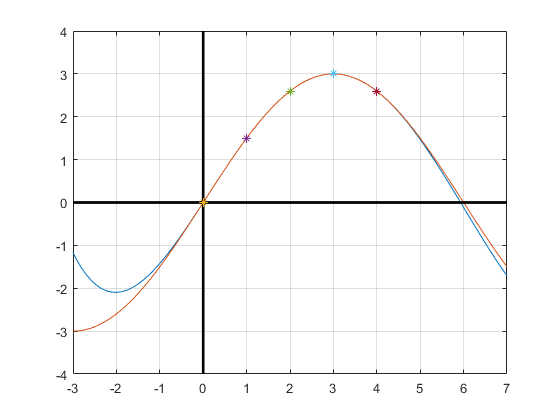
\includegraphics{Images/lagraph.png}
          \caption{Gráfica del polinomio de LaGrange}
          \label{taco}
        \end{figure}
      \end{center}

      Como es posible observar, ambas gráficas, especialmente entre los valores dados, existe una gran cercanía de las 2 gráficas. En este sentido, podemos afirmar que dentro de los puntos dados, la interpolación efectivamente tiene un alto nivel de precisión.

      En cuanto al polinomio de Newton, se desarrolló \texttt{newtong.m} el cual, en términos simples, realiza las mismas instrucciones que \texttt{lagraph.m} pero para el resultado de \texttt{newtonPoly(pointMatrix)}.

      \begin{lstlisting}
syms x

dom = linspace(-3, 7);

orig = @(x) 3 * sin(pi*x/6);

inter = matlabFunction((3*x)/2 - (905051912390271*x*(x - 1))/4503599627370496 - (441695988904705*x*(x - 1)*(x - 2))/9007199254740992 + (8960769158908629*x*(x - 1)*(x - 2)*(x - 3))/1152921504606846976);


plot(dom, inter(dom))
hold on
plot(dom, orig(dom))
hold on
axis([-3, 7, -4, 4])
line([0,0], ylim, 'Color', 'k', 'LineWidth', 2)
line(xlim, [0,0], 'Color', 'k', 'LineWidth', 2) 
grid on

plot(0,orig(0),'*')
plot(1,orig(1),'*')
plot(2,orig(2),'*')
plot(3,orig(3),'*')
plot(4,orig(4),'*')
      \end{lstlisting}

      Tras la ejecución del script, se genera la figura \ref{ugh} en la cual, al igual que con le polinomio de LaGrange, podemos observar el como esta tiene una alta cercanía con la función original.

      \begin{center}
        \begin{figure}[H]
          \centering
          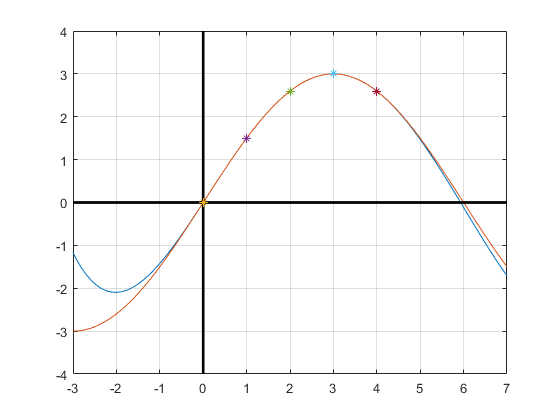
\includegraphics{Images/newtong.png}
          \caption{Gráfica del polinomio de Newton}
          \label{ugh}
        \end{figure}
      \end{center}

      Como es posible apreciar, y al igual que en la figura \ref{taco}, la cercanía entre las 2 gráficas sugiere que las interpolaciones realizadas tienen un alto grado de precisión dentro de los puntos que fueron inicialmente dados para la construcción del polinomio de Newton.
    \end{enumerate}

    \item Interpretando
    
    Para finalizar, se pide encontrar el grado del polinomio de Taylor $P_N(x)$ el cual permita aproximar $\cos(33 \pi / 32)$ para un error menor de $10^{-6}$ cuando $x_o = \pi$. Para realizar esto, debemos partir de la función que nos permite calcular el error de manera inicial. 

    \begin{center}
      \begin{math}
        E_N(x) = \displaystyle \frac{f^{(N+1)}(c)}{(N+1)!} (x-x_0)^{(N+1)}
      \end{math}
    \end{center}

    A partir de esto, podemos realizar algunos remplazos dentro de la ecuación. Lo primero es nuestra función y el valor de x, estos valores pueden ser fácilmente determiados mirando a la ecuación a aproximar. Para $\cos (33 \pi / 32)$, podemos ver que el valor de $x$ es $33 \pi /32$ y que nuestra función es $\cos(x)$. 

    \begin{center}
      \begin{math}
        E_N(\frac{33 \pi}{32}) = \displaystyle \frac{\cos^{(N+1)}(c)}{(N+1)!} \textstyle (\frac{ \pi}{32})^{(N+1)}
      \end{math}
    \end{center}

    Para N = 1 , para c se tomará el valor de $\pi$ puesto es que es el máximo valor que el denominador puede tomar. 

    \begin{center}
      \begin{math}
        E_1(\frac{33 \pi}{32}) = \displaystyle \frac{\cos''(\pi)}{2!} \textstyle (\frac{ \pi}{32})^{(2)}
      \end{math}

      \begin{math}
        E_1(\frac{33 \pi}{32}) = \displaystyle \frac{-\cos(\frac{33 \pi}{32})}{2!} \textstyle (\frac{ \pi}{32})^{(2)} = 0.00453149880662 > 10^{-6}
      \end{math}
    \end{center}

    Para N = 2, c tomará el valor de $\frac{33 \pi}{32}$ para así maximizar nuevamente el error. 

    \begin{center}
      \begin{math}
        E_2(\frac{33 \pi}{32}) = \displaystyle \frac{\cos^{(3)}(\pi)}{(3)!} \textstyle (\frac{ \pi}{32})^{(3)}
      \end{math}

      \begin{math}
        E_2(\frac{33 \pi}{32}) = \displaystyle \frac{\sin(\pi)}{(3)!} \textstyle (\frac{ \pi}{32})^{(3)} = 0.0000140947889013 > 10^{-6}
      \end{math}
    \end{center}

    Para N = 3, c tomará el valor de $\pi$ para así maximizar nuevamente el error. 

    \begin{center}
      \begin{math}
        E_3(\frac{33 \pi}{32}) = \displaystyle \frac{\cos^{(4)}(\pi)}{(4)!} \textstyle (\frac{ \pi}{32})^{(4)}
      \end{math}
    \end{center}

    \begin{center}
      \begin{math}
        E_3(\frac{33 \pi}{32}) = \displaystyle \frac{\cos(\pi)}{(4)!} \textstyle (\frac{ \pi}{32})^{(4)} = 0.00000340593371579 > 10^{-6}
      \end{math}
    \end{center}

    Para N = 4, c tomará el valor de $\frac{33 \pi}{32}$ para así maximizar nuevamente el error. 

    \begin{center}
      \begin{math}
        E_4(\frac{33 \pi}{32}) = \displaystyle \frac{\cos^{(5)}(\frac{33 \pi}{32})}{(5)!} \textstyle (\frac{ \pi}{32})^{(5)}
      \end{math}
    \end{center}

    \begin{center}
      \begin{math}
        E_4(\frac{33 \pi}{32}) = \displaystyle \frac{-\sin(\frac{33 \pi}{32})}{(5)!} \textstyle (\frac{\pi}{32})^{(5)}) = 3.3545519141 \times 10^{-7} < 10^{-6}
      \end{math}
    \end{center}

    Entonces, como podemos ver, el grado para el cual el error de la aproximación de Taylor para $\cos(\frac{33 \pi}{32})$ es N = 4 en donde el error obtenido es $3.3545519141 \times 10^{-7} $.

\end{enumerate}

\newpage

\section{Anexos}

\texttt{lagrangePoly.m}
\begin{lstlisting}
function output = lagrangePoly(pointMatrix)
    
    syms x

    [vS, hS] = size(pointMatrix);

    output = NaN;

    if(hS == 2 && vS > 1) %%Las entradas son correctas cuando los puntos son de (x,y)
        L = [];
        for index = 1:vS
            tempFun = 1;
            for pain = 1:vS
                if(pain == index)
                    %%  Skip!
                else
                    tempFun = tempFun * ((x-pointMatrix(pain,1))/(pointMatrix(index,1) - pointMatrix(pain,1)));
                end
            end
            L = [L tempFun];
        end

        fullFunc = 0;

        for finex = 1:vS
            fullFunc = fullFunc + pointMatrix(finex,2) * L(finex);
        end

        output = fullFunc;

    end

end
\end{lstlisting}

\texttt{newtonPoly.m}
\begin{lstlisting}
function output = newtonPoly(pointMatrix)

    syms x

    [vS, hS] = size(pointMatrix);

    output = NaN;

    if(hS == 2) %%Las entradas son correctas cuando los puntos son de (x,y)

        funTrix = zeros(vS,vS);

        for starex = 1:vS
            funTrix(starex,1) = pointMatrix(starex,2);
        end
        
        for index = 2:vS
            for pain = index:vS
                funTrix(pain,index) = ((funTrix(pain,index-1)-funTrix(pain-1,index-1))/(pointMatrix(pain,1)-pointMatrix((pain - index + 1), 1)));
            end
        end

        fullFunc = funTrix(1,1);
        fullFuncAux = 1;

        for fintrex = 2:vS 
            fullFuncAux = fullFuncAux * (x-pointMatrix(fintrex-1,1));
            fullFunc = fullFunc + funTrix(fintrex, fintrex) * fullFuncAux;
        end

        output = fullFunc;
    end 
end
\end{lstlisting}

\texttt{lagrangeRunner.m}
\begin{lstlisting}
f = @(x) 3 * sin(pi*x/6);
pointMatrix = [0 f(0); 1 f(1); 2 f(2); 3 f(3); 4 f(4)];
  
lagrangeP = lagrangePoly(pointMatrix)
\end{lstlisting}

\texttt{newtonRunner.m}
\begin{lstlisting}
f = @(x) 3 * sin(pi*x/6);
pointMatrix = [0 f(0); 1 f(1); 2 f(2); 3 f(3); 4 f(4)];

newtonP = newtonPoly(pointMatrix)
\end{lstlisting}

\texttt{lagraph.m}
\begin{lstlisting}
syms x

dom = linspace(-3, 7);

orig = @(x) 3 * sin(pi*x/6);

inter = matlabFunction((3*3^(1/2)*x*(x/2 - 2)*(x - 1)*(x - 3))/4 - x*(x/2 - 1/2)*(x - 2)*(x - 4) - (3*x*(x/2 - 3/2)*(x/3 - 4/3)*(x - 2))/2 + (3*3^(1/2)*x*(x/2 - 1)*(x/3 - 1/3)*(x - 3))/8);


plot(dom, inter(dom))
hold on
plot(dom, orig(dom))
hold on
axis([-3, 7, -4, 4])
line([0,0], ylim, 'Color', 'k', 'LineWidth', 2)
line(xlim, [0,0], 'Color', 'k', 'LineWidth', 2) 
grid on

plot(0,orig(0),'*')
plot(1,orig(1),'*')
plot(2,orig(2),'*')
plot(3,orig(3),'*')
plot(4,orig(4),'*')
\end{lstlisting}

\texttt{newtong.m}
\begin{lstlisting}
syms x

dom = linspace(-3, 7);

orig = @(x) 3 * sin(pi*x/6);

inter = matlabFunction((3*x)/2 - (905051912390271*x*(x - 1))/4503599627370496 - (441695988904705*x*(x - 1)*(x - 2))/9007199254740992 + (8960769158908629*x*(x - 1)*(x - 2)*(x - 3))/1152921504606846976);


plot(dom, inter(dom))
hold on
plot(dom, orig(dom))
hold on
axis([-3, 7, -4, 4])
line([0,0], ylim, 'Color', 'k', 'LineWidth', 2)
line(xlim, [0,0], 'Color', 'k', 'LineWidth', 2) 
grid on

plot(0,orig(0),'*')
plot(1,orig(1),'*')
plot(2,orig(2),'*')
plot(3,orig(3),'*')
plot(4,orig(4),'*')

\end{lstlisting}


\end{document}


